\documentclass{scrartcl}

\usepackage{amssymb}
\usepackage{amsmath}
\usepackage{tikz}
\usetikzlibrary{calc,intersections,through,backgrounds,patterns}
\usetikzlibrary{decorations.text, decorations.markings, fit, arrows, arrows.meta}

%replicating Nick Srnicek's diagram, `Neoplatonism versus Nonphilosophy'
%http://speculativeheresy.files.wordpress.com/2010/03/neoplatonism-and-nonphilosophy.jpg

\begin{document}
	
	%\begin{figure}
	%	\centering
	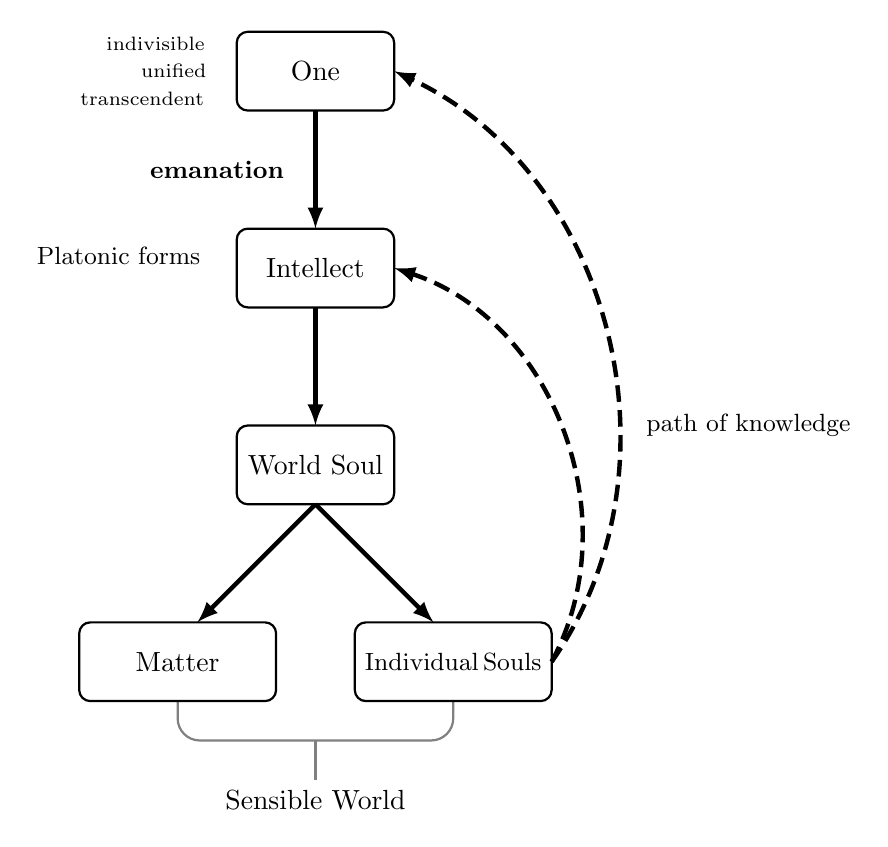
\begin{tikzpicture}
	%bottom bracket
	\draw[gray,thick,rounded corners=8pt] (-1.75,-2.5)--(-1.75,-3)--(1.75,-3)--(1.75,-2.5);
	\draw[gray,thick] (0,-3)--(0,-3.5);
	
	%boxes
	\draw[rounded corners,thick] (-1,0) rectangle (1,1);
	\draw[rounded corners,thick] (-1,2.5) rectangle (1,3.5);
	\draw[rounded corners,thick] (-1,5) rectangle (1,6);
	%
	\draw[rounded corners,thick] (-3,-2.5) rectangle (-0.5,-1.5);
	\draw[rounded corners,thick] (3,-2.5) rectangle (0.5,-1.5);
	
	%inner labels
	\node at (0,0.5)	{World Soul};
	\node at (0,3)		{Intellect};
	\node at (0,5.5)	{One};
	\node at (-1.75,-2)	{Matter};
	\node at (1.75,-2)	{{\small Individual$\,$Souls}};
	\node at (0,-3.75)	{Sensible World};
	
	%arrows
	\draw[->,>=latex,ultra thick] (0,5)--(0,3.5);
	\draw[->,>=latex,ultra thick] (0,2.5)--(0,1);
	\draw[->,>=latex,ultra thick] (0,0)--(-1.5,-1.5);
	\draw[->,>=latex,ultra thick] (0,0)--(1.5,-1.5);
	%
	\draw[->,>=latex,ultra thick,dash pattern=on 6pt off 3pt] (3,-2) to[bend right=50] (1,3);
	\draw[->,>=latex,ultra thick,dash pattern=on 6pt off 3pt] (3,-2) to[bend right=50] (1,5.5);
	
	%outer labels
	\node at (5.5,1)	 {{\small path of knowledge}};
	\node at (-2.5,3.15) {{\small Platonic forms}};
	\node at (-1.25,4.25){{\small \textbf{emanation}}};
	\node at (-2.03,5.85){{\scriptsize indivisible}};
	\node at (-1.8,5.5)  {{\scriptsize unified}};
	\node at (-2.2,5.15) {{\scriptsize transcendent}};
	
	%\draw[help lines] (-3,-3) grid (6,6);
	\end{tikzpicture}
	%	\caption{Plotinus}
	%\end{figure}
	
	
	\vspace{0.8cm}
	
	
	\hspace{-3cm}
	%\begin{figure}
	%	\centering
	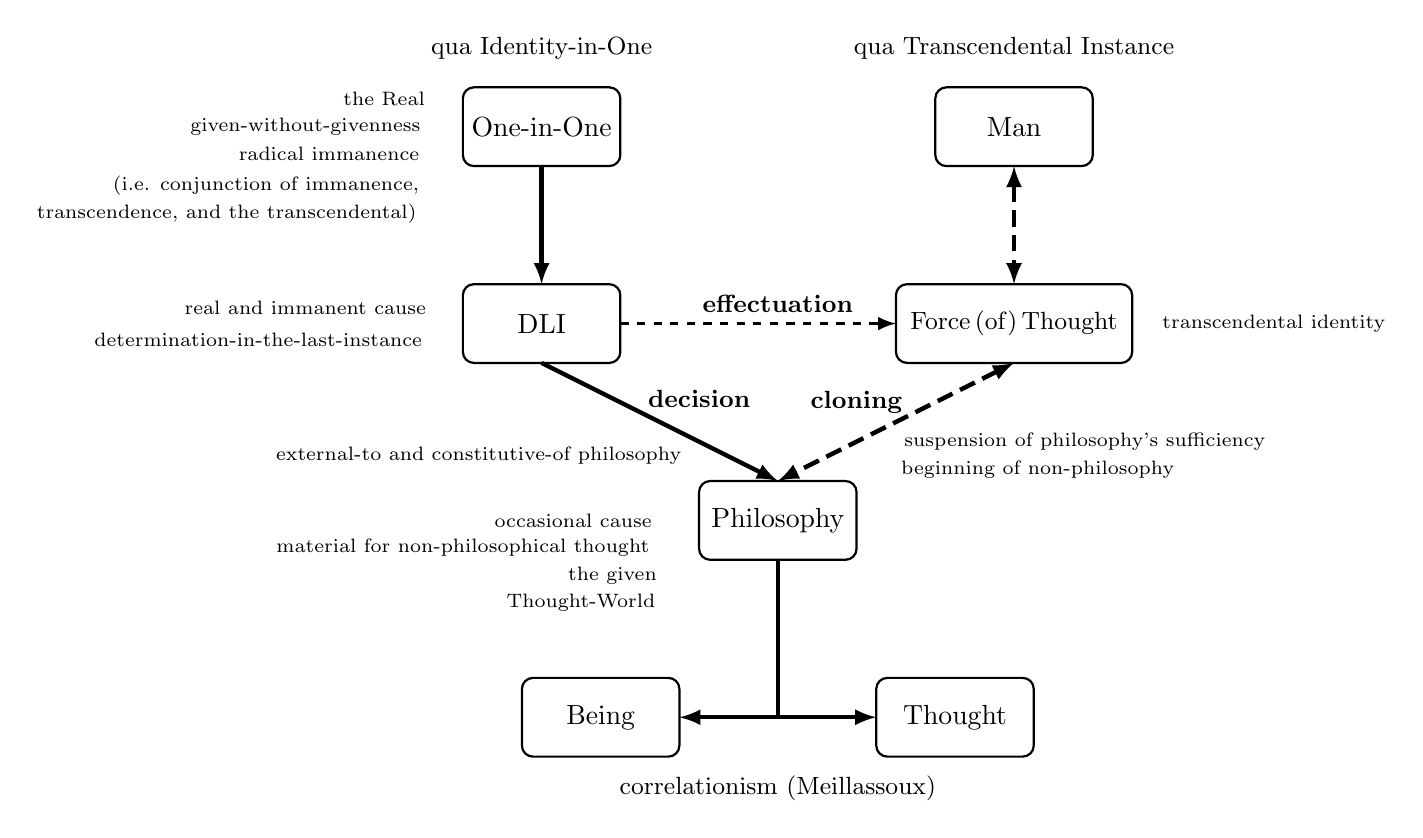
\begin{tikzpicture}
	%boxes
	\draw[rounded corners,thick] (-2,6) rectangle (-4,5);
	\draw[rounded corners,thick] (2,6) rectangle (4,5);
	%
	\draw[rounded corners,thick] (-2,3.5) rectangle (-4,2.5);
	\draw[rounded corners,thick] (1.5,3.5) rectangle (4.5,2.5);
	%
	\draw[rounded corners,thick] (-1,0) rectangle (1,1);
	\draw[rounded corners,thick] (-3.25,-2.5) rectangle (-1.25,-1.5);
	\draw[rounded corners,thick] (3.25,-2.5) rectangle (1.25,-1.5);
	
	%inner labels
	\node at (-3,5.5) {One-in-One};
	\node at (3,5.5)  {Man};
	\node at (-3,3)   {DLI};
	\node at (3,3)	  {{\small Force$\,$(of)$\,$Thought}};
	%
	\node at (0,3.25)  {{\small \textbf{effectuation}}};
	\node at (-1,2.05) {{\small \textbf{decision}}};
	\node at (1,2)     {{\small \textbf{cloning}}};
	%
	\node at (0,0.5)   {Philosophy};
	\node at (-2.25,-2){Being};
	\node at (2.25,-2) {Thought};
	\node at (0,-2.9)  {{\small correlationism (Meillassoux)}};
	
	%arrows
	\draw[->,>=latex,ultra thick] (-3,5)--(-3,3.5);
	\draw[<->,>=latex,ultra thick,dash pattern=on 6pt off 3pt] (3,5)--(3,3.5);
	%
	\draw[ultra thick] (0,0)--(0,-2);
	\draw[<->,>=latex,ultra thick] (-1.25,-2)--(1.25,-2);
	%
	\draw[->,>=latex,ultra thick] (-3,2.5)--(0,1);
	\draw[<->,>=latex,ultra thick,dash pattern=on 6pt off 3pt] (3,2.5)--(0,1);
	%
	\draw[->,>=latex,very thick,dashed] (-2,3)--(1.5,3);	%effectuation
	
	%outer labels
	\node at (-3,6.5) {{\small qua Identity-in-One}};
	\node at (3,6.5)  {{\small qua Transcendental Instance}};
	%
	\node at (-5,5.85)  {{\scriptsize the Real}};
	\node at (-6,5.5)   {{\scriptsize given-without-givenness}};
	\node at (-5.7,5.15){{\scriptsize radical immanence}};
	\node at (-6.5,4.75){{\scriptsize (i.e. conjunction of immanence,}};
	\node at (-7,4.4)   {{\scriptsize transcendence, and the transcendental)}};
	%
	\node at (-6,3.2)   {{\scriptsize real and immanent cause}};
	\node at (-6.6,2.8) {{\scriptsize determination-in-the-last-instance}};
	\node at (6.3,3)	{{\scriptsize transcendental identity}};
	%
	\node at (-3.8,1.325){{\scriptsize external-to and constitutive-of philosophy}};
	\node at (3.9,1.5)	 {{\scriptsize suspension of philosophy's sufficiency}};
	\node at (3.3,1.15)	 {{\scriptsize beginning of non-philosophy}};
	%
	\node at (-2.6,0.5)	  {{\scriptsize occasional cause}};
	\node at (-4,0.15)    {{\scriptsize material for non-philosophical thought}};
	\node at (-2.1,-0.2)  {{\scriptsize the given}};
	\node at (-2.5,-0.55) {{\scriptsize Thought-World}};
	
	%\draw[help lines] (-6,-4) grid (6,6);
	\end{tikzpicture}
	%	\caption{Laruelle}
	%\end{figure}
	
\end{document}